\documentclass{beamer}
\def\presentationtype{0}
\def\corsodilaurea{Ingegneria Informatica e dell'Automazione Industriale}
\def\insegnamento{Ottimizzazione}
\def\nolezione{8}
\def\titolo{Il metodo del simplesso -- Il ``tableau'' e l'operazione ``pivot''}
\def\noattivita{1}

\def\argomenti{Programmazione Lineare}
\def\obiettivilezione{Definire il ``tableau'' e l'operazione ``pivot'' per poter sviluppare metodo del simplesso primale}
\def\nucleotematico{Richiami}
\def\contenuto{Programmazione lineare}


\usepackage[italian]{babel}
%
% Hyperref info for PDF
%
\usepackage{hyperref}
\hypersetup{%
%pdfpagemode=FullScreen,
pdfpagemode=FullScreen,
pdfstartview=Fit,
pdfsubject={\argomenti},
pdfkeywords={\insegnamento,\titolo}
}

\definecolor{ecampus@engred}{RGB}{227,28,23}
\setbeamercolor{normal text}{fg=black,bg=}
\setbeamercolor{alerted text}{fg=red}
\setbeamercolor{example text}{fg=green!50!black}
\setbeamercolor{structure}{fg=ecampus@engred,bg=}
\usetheme{default}
\useinnertheme{rounded}%{circles}
\setbeamertemplate{blocks}[default]
\setbeamercolor{block title}{bg=}
\setbeamercolor{block body}{bg=}

\ifnum\presentationtype>0 {\setbeamertemplate{enumerate item}{Es. \nolezione.\presentationtype.\arabic{enumi})}} \fi

%\setbeamertemplate{frametitle continuation}[from second][(cont'd)]
\usefonttheme[stillsansseriftext,stillsansserifsmall]{serif}
\setbeamertemplate{headline}{%
\leavevmode%
   \hspace*{4.75cm}
   \scalebox{0.90}{%
    \begin{minipage}{\linewidth}%
      \tiny
 	\begin{tabular}{ll}
	  \\
% 	  \textcolor{gray}{Classe}					& \corsodilaurea\\
%	  \textcolor{gray}{Argomento:}					& \insegnamento\\
%	  \textcolor{gray}{Lezione n}:							& \nolezione \\
	  \textcolor{gray}{Titolo:}			& \titolo \\
	  \textcolor{gray}{Attivit\`a}:		& 	  \ifnum\presentationtype=0 {Lezione \nolezione} \else {Sessione di studio \nolezione.\presentationtype} \fi
	\end{tabular}%
    \end{minipage}%
   }%
}
\setbeamertemplate{footline}[text line]{%
  \begin{minipage}{\linewidth}%
    \hfill\insertpagenumber%
%    
    \begin{center}%
      \rule{\linewidth}{0.4pt}
    \end{center}
    \vspace*{-0.65cm}
    \begin{center}%
      \scalebox{0.55}{%
	\begin{minipage}{\linewidth}%
	  \begin{center}%
	    {\tiny
	    \copyright \ 2022 Gionata Massi - \color{blue}{\href{mailto:gionata.massi@savoiabenincasa.it}{gionata.massi@savoiabenincasa.it}}\\
	    \phantom{XXX}}
	  \end{center}
	\end{minipage}%
      }%
    \end{center}%
%
  \end{minipage}%
  }
\setbeamertemplate{navigation symbols}{}

%% Save up on ink for the 4-up handouts
\mode<handout>{%
  \pgfpagesuselayout{4 on 1}[a4paper, landscape, border shrink=10mm]
  \pgfpageslogicalpageoptions{1}{border code=\pgfstroke}
  \pgfpageslogicalpageoptions{2}{border code=\pgfstroke}
  \pgfpageslogicalpageoptions{3}{border code=\pgfstroke}
  \pgfpageslogicalpageoptions{4}{border code=\pgfstroke}
}

\mode<presentation>{\AtBeginSection{%
  \begin{frame}
    \frametitle{Piano della presentazione}
    \tableofcontents[currentsection]
  \end{frame}}
}

\usepackage{microtype}
\usepackage[utf8]{inputenc}
\usepackage[T1]{fontenc}
%\usepackage[osfss]{libertine}
\usepackage{palatino}
\usepackage[scaled=.77]{beramono}
\usepackage{booktabs}
% \usepackage{attachfile}

% Toglie l'enorme spazione prima di description
%\setbeamersize{description width=0pt}

\usepackage{tikz}
\usetikzlibrary{decorations,arrows,shapes,backgrounds,matrix,positioning}
\usepackage{multirow}
\usepackage{verbatim}
\usepackage{eurosym}
\usepackage{pgfpages}

\usepackage{zref-savepos}
\newcounter{restofframe}
\newsavebox{\restofframebox}
\newlength{\mylowermargin}
\setlength{\mylowermargin}{2pt}

\newenvironment{restofframe}{%
    \par%\centering
    \stepcounter{restofframe}%
    \zsavepos{restofframe-\arabic{restofframe}-begin}%
    \begin{lrbox}{\restofframebox}%
}{%
    \end{lrbox}%
    \setkeys{Gin}{keepaspectratio}%
    \raisebox{\dimexpr-\height+\ht\strutbox\relax}[0pt][0pt]{%
    \resizebox*{!}{\dimexpr\zposy{restofframe-\arabic{restofframe}-begin}sp-\zposy{restofframe-\arabic{restofframe}-end}sp-\mylowermargin\relax}%
        {\usebox{\restofframebox}}%
    }%
    \vskip0pt plus 1filll\relax
    \mbox{\zsavepos{restofframe-\arabic{restofframe}-end}}%
    \par
}

\title{\titolo}
\author{Gionata Massi}
\date{\today}

\setbeamercolor*{frametitle}{fg=black}
\setbeamercolor*{title}{fg=black}
\setbeamerfont{frametitle}{shape=\scshape,family=\rmfamily,size=\large,series=\bfseries}

\setbeamersize{}
\makeatletter
\newcommand\thefontsize[1]{{#1 The current font size is: \f@size pt\par}}
\makeatother

\tikzstyle{nicebox}=[draw=gray!100, fill=blue!10, very thick,
rounded corners, rectangle, inner sep=4pt, inner ysep=16pt]
\tikzstyle{niceboxtitle}=[draw=gray!100, fill=white, text=black,
rounded corners, very thick, rectangle]
\newcommand\nicebox[2]{
{\centering
\begin{tikzpicture}
\node [nicebox](box){
\begin{minipage}{0.95\textwidth}\centering
\begin{minipage}{0.95\textwidth}
#2
\end{minipage}\end{minipage}};
\node[niceboxtitle, right=10pt] at (box.north west)
{\small\textbf{#1}};
\end{tikzpicture}\par}
}

\tikzstyle{modelbox}=[draw=structure!100, fill=white!50, very thick,
rounded corners, rectangle, inner sep=4pt, inner ysep=16pt, text=blue!50!black]
\tikzstyle{modelboxtitle}=[draw=structure!100, fill=white!50, text=blue!50!black,
rounded corners, very thick, rectangle]
\newcommand\modelbox[2]{
{\centering
\begin{tikzpicture}
\node [modelbox](box){
\begin{minipage}{0.95\textwidth}\centering
\begin{minipage}{0.95\textwidth}
#2
\end{minipage}\end{minipage}};
\node[modelboxtitle, right=10pt] at (box.north west)
{\small\textbf{\mbox{#1}}};
\end{tikzpicture}\par}
}

% % %
% Tipi di sessioni di studio
% % %
\def\domande{Domande}
\def\approfondimenti{Approfondimenti}
\def\esercizi{Esercizi}
\def\esempi{Esempi svolti}
\def\relazioni{Relazioni}
\def\attivitapratica{Attivit\`a pratica}
% % %

\newcommand{\generatitolo}{ %
\begin{frame}[plain]
\pdfbookmark{\ifnum\presentationtype=0 {Lezione \nolezione} \else {Sessione di studio \nolezione.\presentationtype} \fi}{\ifnum\presentationtype=0 {Lezione \nolezione} \else {Sessione di studio \nolezione.\presentationtype} \fi}
\noindent\hspace*{3.715cm}
   \scalebox{0.90}{%
    \begin{minipage}{\linewidth}%
      \tiny
 	\begin{tabular}{ll}
	  \\
% 	  \textcolor{gray}{Classe}					& \corsodilaurea\\
%	  \textcolor{gray}{Argomento:}					& \insegnamento\\
%	  \textcolor{gray}{Lezione n}:							& \nolezione \\
	  \textcolor{gray}{Titolo:}			& \titolo \\
	  \textcolor{gray}{Attivit\`a}:		& 	  \ifnum\presentationtype=0 {Lezione \nolezione} \else {Sessione di studio \nolezione.\presentationtype} \fi
	\end{tabular}%
    \end{minipage}%
   }%
   
  \begin{center}
    \large{\textbf{\insegnamento}}
  \end{center}

  \vspace*{0.5cm}
  
  \begin{center}
    \huge{\titolo}
  \end{center}
  
  \begin{center}
	  \ifnum\presentationtype=0
	    {Lezione n$^{\circ}$ \nolezione}
	  \else
	    {Sessione di studio n$^{\circ}$ \nolezione .\presentationtype}
	  \fi
  \end{center}
  
  \vspace*{0.5cm}

  \begin{center}
    \large{\textsl{Gionata Massi}}\\
    \scriptsize\color{blue}{<\href{mailto:gionata.massi@savoiabenincasa.it}{gionata.massi@savoiabenincasa.it}>}
  \end{center}
  
  \newcounter{pageleft}
  \zsaveposy{pageleft}
  \vspace*{\dimexpr\zposy{pageleft}sp-1.67cm}

  \begin{minipage}{\linewidth}%
   \hfill\phantom{\insertpagenumber}%

  \begin{center}%
      \rule{\linewidth}{0.4pt}
    \end{center}
    
    \vspace*{-0.95cm}
    
    \begin{center}%
      \scalebox{0.55}{%
	\begin{minipage}{\linewidth}%
	  %\begin{center}%
	  %  \tiny
	  %  \copyright \ 2022 Gionata Massi - \color{blue}{\href{mailto:gionata.massi@savoiabenincasa.it}{gionata.massi@savoiabenincasa.it}}\\
	  %  \color{blue}{\href{mailto:gionata.massi@savoiabenincasa.it}{gionata.massi@savoiabenincasa.it}}\\
	  %  \phantom{XXX}
	  %\end{center}
	\end{minipage}%
      }%
    \end{center}%
     \phantom{XXX}
%
  \end{minipage}%

\end{frame}
}

\renewcommand{\vec}{\mathbf}
\newcommand{\matr}{\mathbf}

\uselanguage{italian}
\languagepath{italian}
\deftranslation[to=italian]{Theorem}{Teorema}
\deftranslation[to=italian]{theorem}{teorema}
\deftranslation[to=italian]{Definition}{Definizione}
\deftranslation[to=italian]{definition}{definizione}
\deftranslation[to=italian]{Corollary}{Corollario}
\deftranslation[to=italian]{corollary}{corollario}

\let\definition\relax
\let\enddefinition\relax

%\theoremstyle{example}
\newtheorem{definition}[theorem]{\translate{Definition}}

\def\fieldN{\mathbb{N}}
\def\fieldR{\mathbb{R}}
\def\fieldZ{\mathbb{Z}}

\def\matrA{\matr{A}}
\def\vecB{\vec{b}}
\def\vecC{\vec{c}}
\def\vecX{\vec{x}}

\usepackage{cancel}
\usepackage{bookmark}

% tkiz ball item
\newcommand*\circled[1]{\raisebox{2.5pt}{\tikz[baseline=(char.base)]{
            \node[circle,ball color=purple, shade, 
 color=white,inner sep=1.2pt] (char) {\tiny #1};}}}

% tkiz rounded item
\newcommand*\rounded[1]{\tikz[baseline=(char.base)]{
            \node[draw=none,ball color=purple, shade, 
 color=white, rounded corners=3.5pt, inner sep=2.5pt] (char) {\scriptsize #1};}}

 \usepackage{etoolbox}
\makeatletter
\apptocmd{\beamer@@frametitle}{\write\@auxout{\string\@writefile{frm}{\string\frametitleentry{\the\c@framenumber}{#1}{#2}}}}{}{}
\newcommand*{\frametitleentry}[3]{\@namedef{frametitleshort#1}{#2}\@namedef{frametitle#1}{#3}}
\AtEndDocument{\if@filesw\newwrite\tf@frm\immediate\openout\tf@frm\jobname.frm\relax\fi}
\@input{\jobname.frm}
\makeatother
 
%\usebackgroundtemplate{
\includegraphics[width=\paperwidth]{../img/sfondo_ecampus.png}}

\usepackage{listings}
% Extension for listings package
\lstdefinelanguage{ampl}{
  % See AMPL book (1993 edition), Appendix A
  morekeywords={%
    % Table A.1
    % Excluding symbols and "not X", where X (and not) are keywords
    if, then, else, or,  exists, forall,  and, in, within, 
    not, union, diff, symdiff, inter, cross, setof, by, 
    % Skipping: less,  sum, prod, min, max, div, mod,
    % Skipping built-in functions (Tables A-2 and A-3)
    % Section A.5 -- Declarations of model entities (subject to ->
    % subject, to)
    set, param, var, arc, minimize, maximize, subject, to, node,
    % Section A.6 -- Set declarations (not repeating set or within)
    dimen, default, card, ordered, by, reversed, circular,
    % Section A.7 -- Parameter declarations (not repeating in, default)
    param, binary, integer, symbolic, check, Infinity
    % Section A.8 -- Variable declarations
    var,  coeff, cover, obj,
    % Section A.13 -- Command language
    % Skipping most commands!
    include, model, data, let, objective, drop, restore, solve,
    solution, quit, end, option, reset, update, commands,
    % A.14 -- Imported functions
    function, pipe, 
    % A.17 synonyms for previously-defined keywords
    coef, difference, dimen, dimension, intersect, intersection, s.t., 
    % 
    % must be defined somewhere ...
    for, while, repeat, break,
    % NEW language features (http://www.ampl.com/NEW/newlang.html)
    % Grouped by page
    purge, problem, redeclare, xref,
    complements, 
    table, IN, OUT, INOUT, read, write, 
    expand,
    for, commands, repeat, until, while, break, continue,
  },
  sensitive=true,
  comment=[l]{\#},
  morecomment=[s]{/*}{*/},
  string=[b]",
  morestring=[b]',
}[keywords,comments,strings]

\definecolor{comment_c}{RGB}{60,128,49}
\definecolor{rowname_c}{RGB}{128,60,49}
\definecolor{reserved_c}{RGB}{49,60,128}

\lstset{
	language=ampl,%
	commentstyle=\color{comment_c},%
	backgroundcolor=\color{blue!15},%
    basicstyle=\small\ttfamily,%
    %emph={s.t.},emphstyle={\bfseries},%
    otherkeywords={s.t.},%
    numbers=left, numberstyle=\tiny, stepnumber=1, numbersep=5pt,%
}

\definecolor{col_set}{RGB}{128,0,0}
\definecolor{col_par}{RGB}{91,0,91}
\definecolor{col_idx}{RGB}{0,91,91}
\definecolor{col_var}{RGB}{0,0,128}

\def\insieme{%1}{\rm \textcolor{col_set}{%1}}}

%\usepackage{amsmath,amssymb,paralist,mathrsfs}


%\pgfdeclareimage[width=5cm,height=2.8cm]{goalsym}{goalsym}
%***SET OF REAL NUMBERS*********
\newcommand{\Rset}{{\mathbb{R}}}
%***SET OF RATIONAL NUMBERS*********
\newcommand{\Qset}{{\mathbb{Q}}}
\def\half{{\textstyle {1\over2}}}
\newcommand{\Nset}{{\mathbb{N}}}
\newcommand{\Parset}{{\mathfrak{C}}}
\newcommand{\Fset}{{\mathscr{F}}}


\begin{document}

\generatitolo

\section{GNU Linear Programming Kit (GLPK)}

\begin{frame}{Informazioni generali}
\begin{itemize}
\item \alert{GNU Linear Programming Kit (GLPK)}:
 \`e un pacchetto software che comprende:
   \begin{itemize} 
	 \item un insieme di routine organizzate come libreria (\texttt{glpk})
	 per problemi PL, PLI e ottimizzazione su rete;
	 \item un programma che permette di inserire e risolvere un modello di programmazione lineare (\texttt{glpsol}) senza dover ricorrere alla programmazione;
	 \item un linguaggio di modellizzazione \structure{GNU MathProg}.
   \end{itemize}
  \item  Il software \'e libero e multipiattaforma
\end{itemize}    
\end{frame}

%\subsection{Istallazione}

\begin{frame}{Installazione del pacchetto GLPK}
   \begin{itemize}
   \item GNU/Linux
	   \begin{itemize}
	   	\item le principali distribuzioni GNU/Linux comprendono un paccetto GLPK (GNU Linear Programming Kit);
	   	\item in altenativa occorre compilare il pacchetto GLPK da \alert{codice sorgente}:
    \href{http://www.gnu.org/software/glpk/glpk.html}{\structure{http://www.gnu.org/software/glpk/glpk.html}}
   \end{itemize}

   \item Windows
   \begin{itemize}
   	   \item GUSEK (GLPK Under Scite Extended Kit): GLPK e ambiente di sviluppo (IDE) -- Windows:
   \href{http://gusek.sourceforge.net/}{\structure{http://gusek.sourceforge.net/}},
%   \item GLPK (GNU Linear Programming Kit) per Windows (senza IDE):
%    \href{http://gnuwin32.sourceforge.net/packages/glpk.htm}{\structure{http://gnuwin32.sourceforge.net/packages/glpk.htm}},
   \end{itemize}

   \item Web browser con supporto Javascript
	\begin{itemize}
	\item collegarsi alla pagina \href{http://www3.nd.edu/~jeff/mathprog/mathprog.html}{\structure{http://www3.nd.edu/\textasciitilde{}jeff/mathprog/mathprog.html}}
	\end{itemize}
\end{itemize} 
\end{frame}

\begin{frame}{Installazione GUSEK (per Windows)}
\begin{enumerate}
\item download (\href{http://gusek.sourceforge.net/}{\structure{http://gusek.sourceforge.net/}});
\item estrazione dei file dall'archivio in una cartella qualsiasi;
\item avvio del file \texttt{gusek.exe}
\end{enumerate}
\end{frame}

\section{Sintassi di base}

\begin{frame}{Caratteristiche generali sintassi GNU MathProg}
\begin{itemize}
\item \`e un linguaggio case sensitive, cio\`e distingue le lettere
maiuscole dalla minuscole;
\item le righe del programma hanno una lunghezza massima di 255 caratteri;
\item i commenti sono introdotti dal simbolo \# e terminano a fine riga, oppure sono compresi tra ``/*'' e ``*/'';
\item le istruzioni del programma sono separate dal simbolo ``;'';
\item ``a capo'' e tabulazioni vengono interpretati come semplici spazi bianchi;
\end{itemize}
\end{frame}

\subsection{Variabili}

\begin{frame}[allowframebreaks]{Variabili}
\noindent
\framebox{
\parbox[c][24pt]{0.85\textwidth}{
\hspace{6pt} {\tt var} {\it name} {\it alias} {\it domain} {\tt,}
{\it attrib} {\tt,} \dots {\tt,} {\it attrib} {\tt;}
}}

\medskip

\begin{description}
\item[{\it name}] \`e il ``nome'' che identifica la variabile;

\item[{\it alias}] opzionale, \`e un altro nome che pu\`o essere associato alla variabile;

\item[{\it domain}] opzionale, \`e un'espressione che specifica il dominio della variabile;

\item[{\it attrib}, \dots, {\it attrib}] opzionali, sono degli attributi che possono essere associati alle variabili per meglio specificale:
{\footnotesize \begin{description}
\item[{\tt integer}]\hspace*{0pt}\\
variabile intera;
\item[{\tt binary}]\hspace*{0pt}\\
variabile binaria (detta anche 0/1);
\item[{\tt>=} {\it espressione}]\hspace*{0pt}\\
specifica il valore minimo che la variabile pu\`o assumere;
\item[{\tt<=} {\it espressione}]\hspace*{0pt}\\
specifica il valore massimo che la variabile pu\`o assumere;
\item[{\tt=} {\it espressione}]\hspace*{0pt}\\
fissa il valore della variabile;
\end{description}}
\end{description}
\end{frame}

\subsection{Funzione obiettivo}

\begin{frame}%[allowframebreaks]
{Funzione obiettivo}
\noindent
\framebox{
\parbox[c][44pt]{0.85\textwidth}{
\hspace{6pt} {\tt minimize} {\it name} {\it alias} {\it domain} {\tt:}
{\it expression} {\tt;}

\medskip

\hspace{6pt} {\tt maximize} {\it name} {\it alias} {\it domain} {\tt:}
{\it expression} {\tt;}
}}

\begin{description}
\item[{\it name}] \`e il ``nome'' dell'obiettivo;

\item[{\it alias}] opzionale, \`e un altro nome per riferirsi alla f.o.;

\item[{\it domain}] optionale, specifica il dominio della f.o.;

\item[{\it expression}] \`e la forma lineare usata per calcolare il
valore della funzione obiettivo.
\end{description}
\end{frame}

\subsection{Vincoli}

\begin{frame}[allowframebreaks]{Vincoli}
\noindent
\framebox{
\parbox[c][106pt]{0.85\textwidth}{
\hspace{6pt} {\tt s.t.} {\it name} {\it alias} {\it domain} {\tt:}
{\it expr} {\tt,} {\tt=} {\it expr} {\tt;}

\medskip

\hspace{6pt} {\tt s.t.} {\it name} {\it alias} {\it domain} {\tt:}
{\it expr} {\tt,} {\tt<=} {\it expr} {\tt;}

\medskip

\hspace{6pt} {\tt s.t.} {\it name} {\it alias} {\it domain} {\tt:}
{\it expr} {\tt,} {\tt>=} {\it expr} {\tt;}

\medskip

\hspace{6pt} {\tt s.t.} {\it name} {\it alias} {\it domain} {\tt:}
{\it expr} {\tt,} {\tt<=} {\it expr} {\tt,} {\tt<=}
{\it expr} {\tt;}

\medskip

\hspace{6pt} {\tt s.t.} {\it name} {\it alias} {\it domain} {\tt:}
{\it expr} {\tt,} {\tt>=} {\it expr} {\tt,} {\tt>=}
{\it expr} {\tt;}
}}

%\medskip
\framebreak

\begin{description}
\item[{\it name}] \`e il ``nome'' del vincolo;

\item[{\it alias}] opzionale, \`e un altro nome del vincolo;

\item[{\it domain}] opzionale, specifica il dominio del vincolo;

\item[{\it expr}] \`e la forma lineare usata per calcolare una componente
del sistema dei vincoli.
\end{description}
\noindent
(La keyword {\tt s.t.} pu\`o essere scritta per esteso come {\tt subject to} oppure come {\tt subj to}, oppure ancora essere omessa)
\end{frame}

\section{Esempio}

\begin{frame}[allowframebreaks]{I programmi lineari}  
\begin{align*}
     \min (\max) & \sum_{j=1}^{n}\textcolor{structure}{c_j} \textcolor{blue}{x_j} && \quad \text{ funzione obiettivo}\\
      &\sum_{j=1}^{n} \textcolor{structure}{a_{ij}} \textcolor{blue}{x_j} \lesseqgtr\textcolor{structure}{b_i},  & i=1,\ldots, m&\quad \text{  vincoli }\\
      &\textcolor{blue}{x_j}\geq 0,  &j=1,\ldots, n& \quad \text{ var. non negative}
\end{align*}
\hfil{\color{blue} \rule{1em}{1em} variabili}\hspace*{1cm}{\color{red} \rule{1em}{1em} parametri}\hfil

{\bf Nota}: il simbolo "$\lesseqgtr$" viene usato per indicare che il vincolo pu\`o essere sia di eguaglianza ($=$) che di diseguaglianza ($\leq$ o  $\geq$).

\begin{itemize}
\item Parametri (dati in ingresso):
     \begin{itemize}
        \item $c_j$, $j=1,\ldots, n$, coefficienti della funzione obiettivo,
        \item  $b_i$, $i=1,\ldots, m$, termini noti,
        \item $a_{ij}$, $i=1,\ldots, m$,  $j=1,\ldots, n$, matrice dei coefficienti tecnologici. 
     \end{itemize}
\item $x_j$,  $j=1,\ldots, n$, variabili decisionali (uscita).    
\end{itemize}
\end{frame}


\begin{frame}[allowframebreaks,fragile]{Esempio: un'istanza di mix di produzione}
%\structure{\bf Un programma lineare: un'istanza di mix di produzione ottimale}
\[
\begin{array}{lrcrlll} 
               \max z = & 120 x_1&+& 40 x_2\\ 
                        &  40 x_1&+& 20 x_2&\leq & 2200\\
                        &   8 x_1&+&  2 x_2&\leq &  320 \\ 
                        &     x_1&+&    x_2&\leq &  100 \\ 
                        & \multicolumn{5}{l}{x_1   \geq  0, x_2 \geq 0} 
\end{array}
\]

\lstinputlisting{allegati/modello_istanziato.mod}

\begin{itemize}
\item Salvare il file come \texttt{modello\_instanziato.mod};
\item risolvere, usando glpsol da linea di comando:
	\begin{itemize}
	\item \verb=glpsol --model feasible.mod=
	\item \verb=glpsol --model feasible.mod --output feasible.txt=
	\end{itemize}
\end{itemize}
\end{frame}

\subsection{Risoluzione utilizzando l'intefaccia Gusek}

\begin{frame}{Inserire il problema in Gusek}
\begin{center}
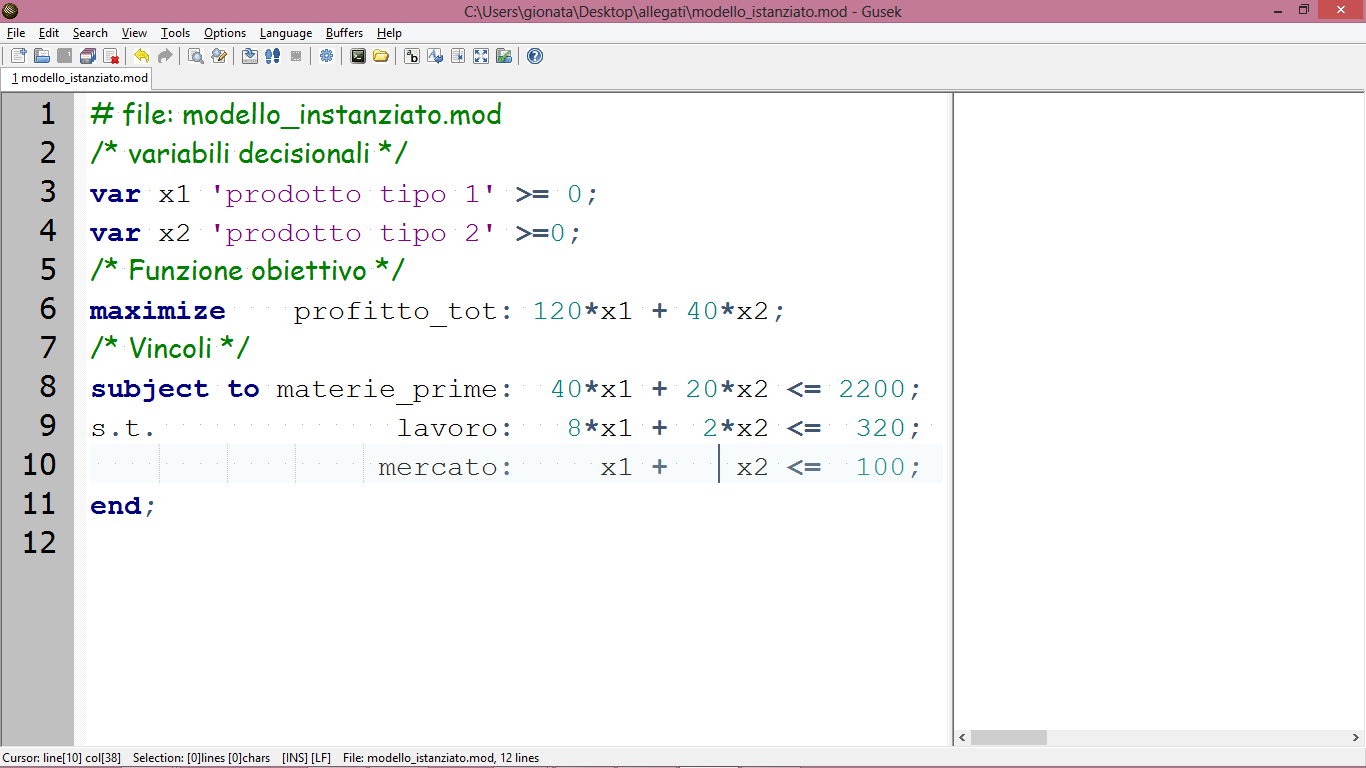
\includegraphics[height=0.85\textheight]{img/gusek_1}
\par\end{center}
\end{frame}

\begin{frame}{Eseguire il risolutore (tasto F5)}
\begin{center}
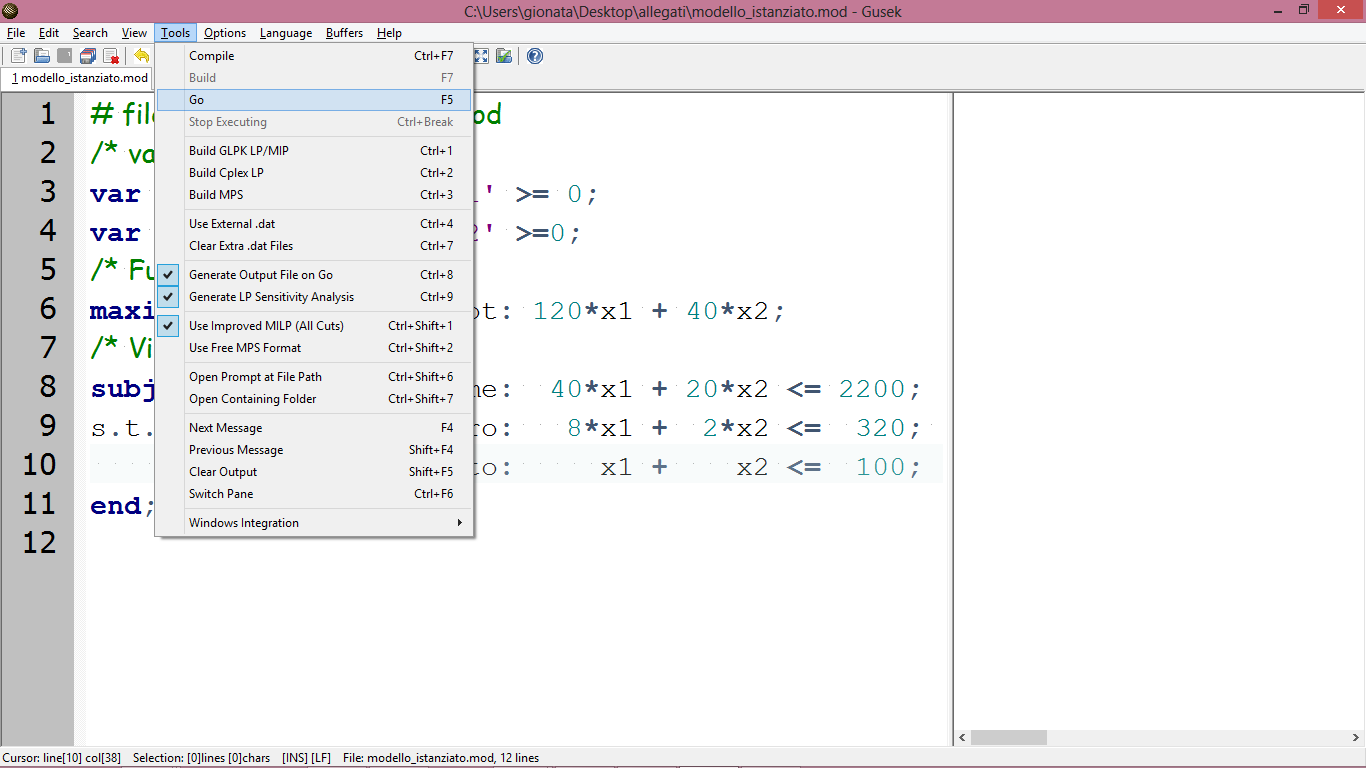
\includegraphics[height=0.85\textheight]{img/gusek_2}
\par\end{center}
\end{frame}

\begin{frame}{Visualizzazione della soluzione}
\begin{center}
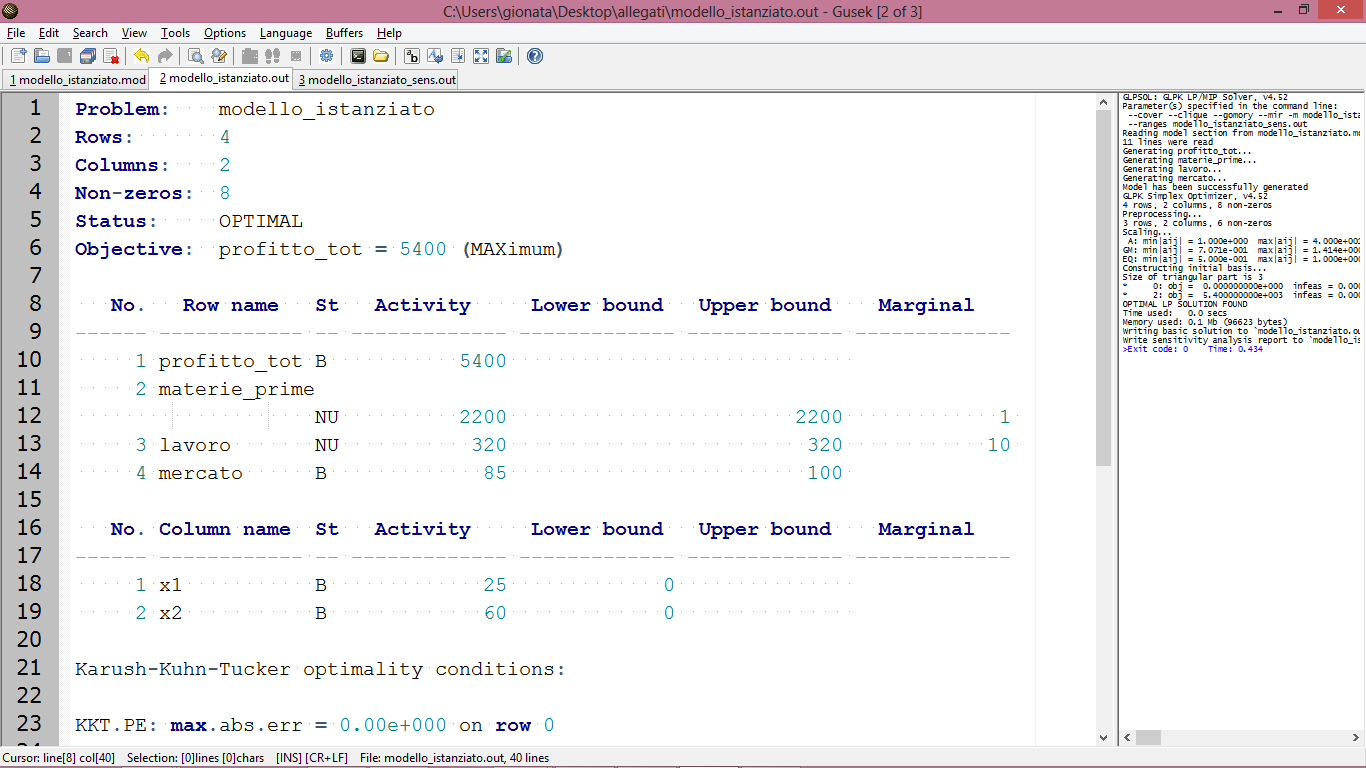
\includegraphics[height=0.85\textheight]{img/gusek_3}
\par\end{center}
\end{frame}

\begin{frame}{Visualizzazione dell'analisi post-ottimale}
\begin{center}
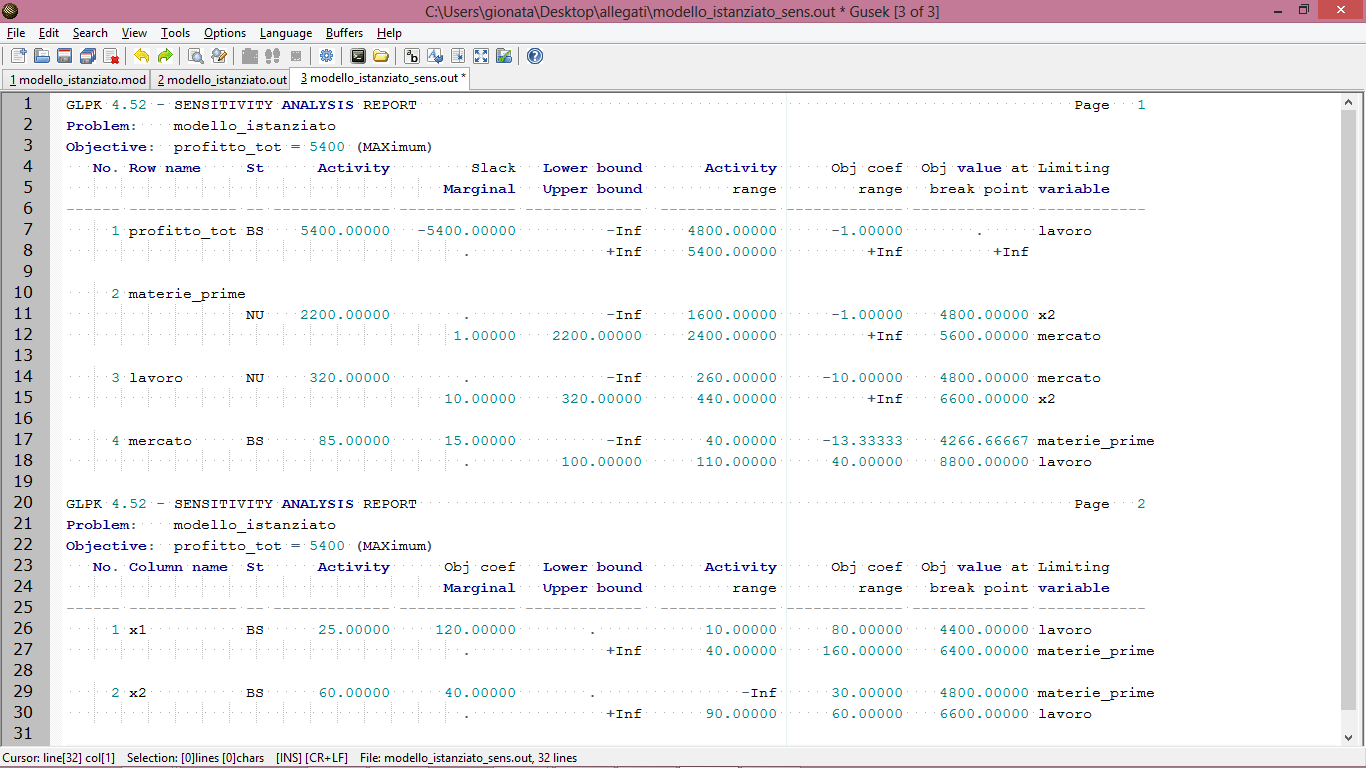
\includegraphics[height=0.85\textheight]{img/gusek_4}
\par\end{center}
\end{frame}

\subsection{Risoluzione utilizzando l'intefaccia Web}

\begin{frame}{Inserire il problema sul sito MathProg}
\begin{center}
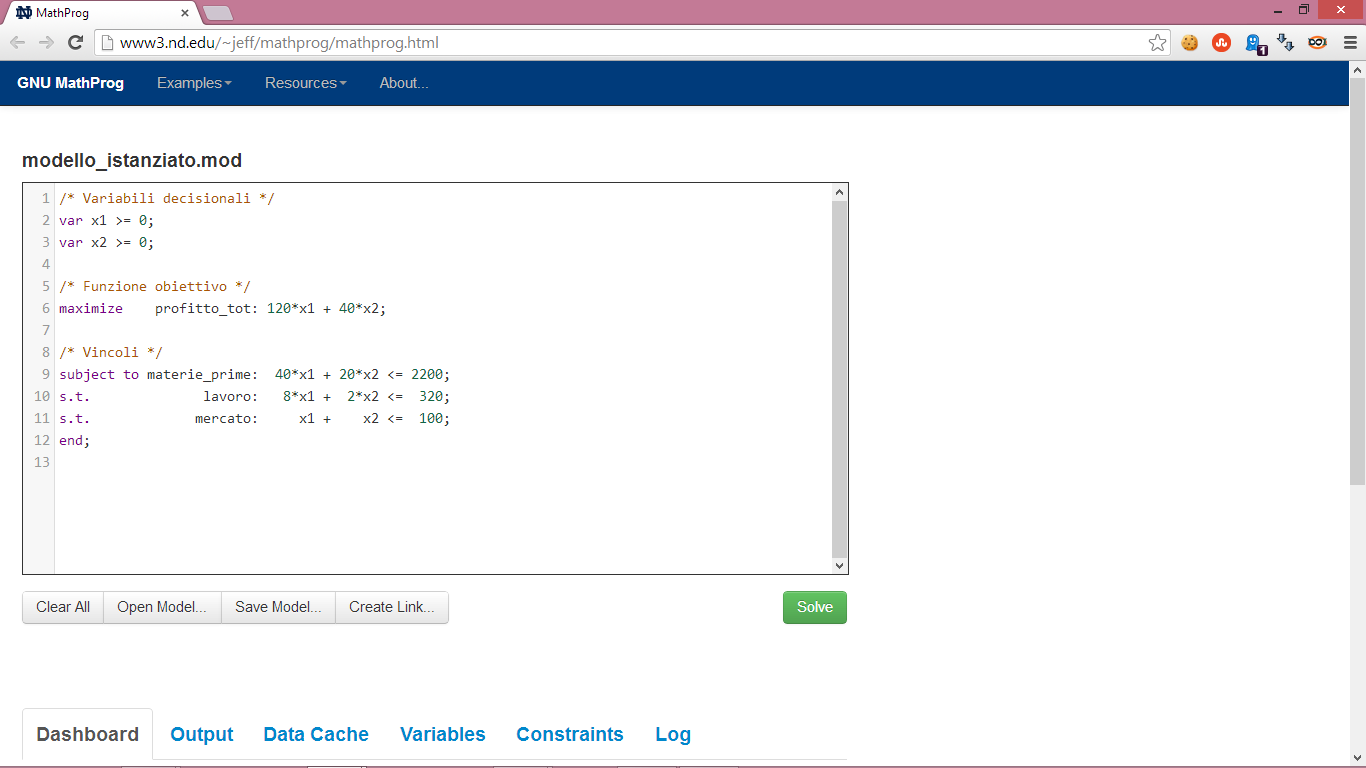
\includegraphics[height=0.85\textheight]{img/mathprog_jeff_1}
\par\end{center}
\end{frame}

\begin{frame}{Eseguire il risolutore (bottone ``Solve'')}
\begin{center}
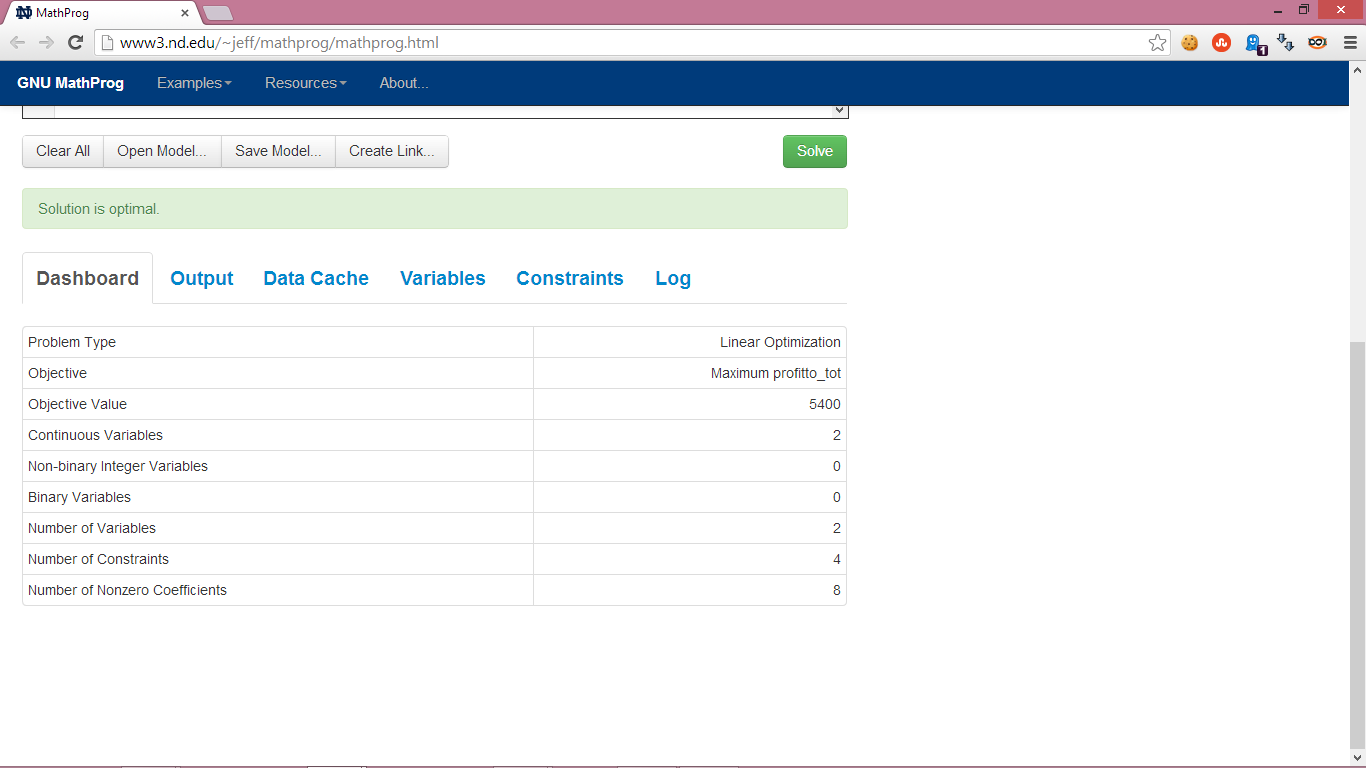
\includegraphics[height=0.85\textheight]{img/mathprog_jeff_2}
\par\end{center}
\end{frame}

\begin{frame}{Visualizzazione della soluzione - variabili}
\begin{center}
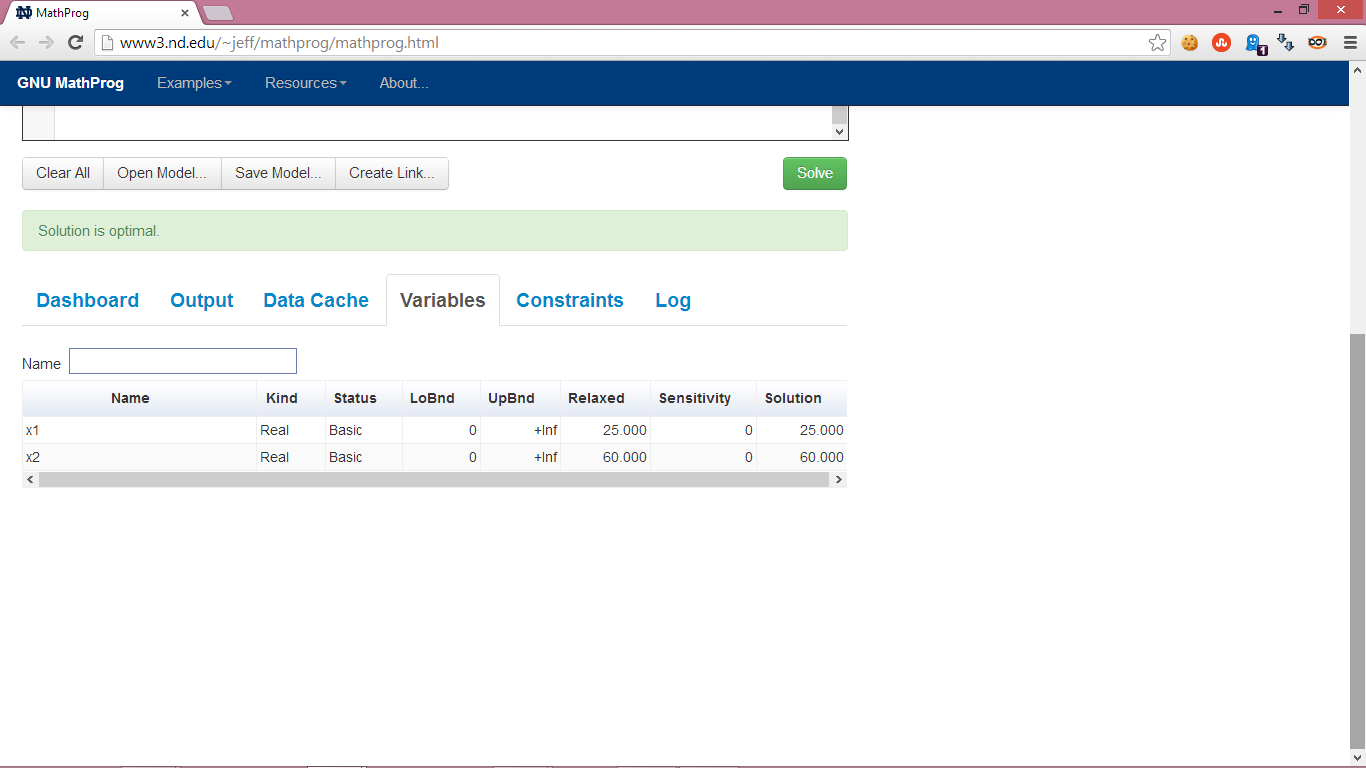
\includegraphics[height=0.85\textheight]{img/mathprog_jeff_3}
\par\end{center}
\end{frame}

\begin{frame}{Visualizzazione della soluzione - vincoli}
\begin{center}
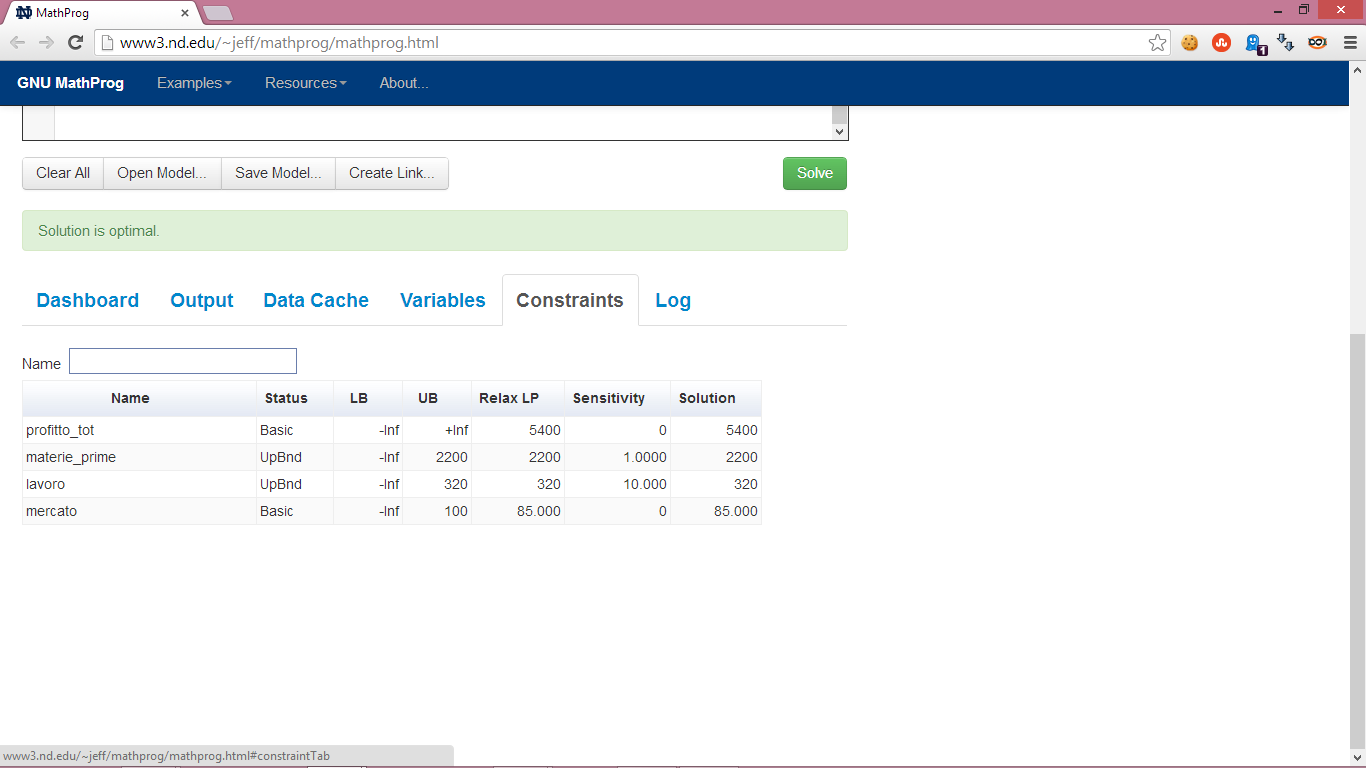
\includegraphics[height=0.85\textheight]{img/mathprog_jeff_4}
\par\end{center}
\end{frame}

\end{document}

\begin{frame}[fragile]
  \frametitle{Linear programming problem}
  \vspace{-0.5cm}
\structure{\bf Example~2:}
\begin{small}
Solve the following linear programming problem:
\[
\begin{array}{rcrlll} 
               \multicolumn{5}{l}{4x_1+2x_2\rightarrow \max}\\ 
                                            x_1&+&x_2&= &40\\
                                            x_1&+&x_2&\geq&120 \\ 
                                 \multicolumn{5}{l}{x_1   \geq  0, x_2 \geq 0} 
\end{array}
\]
The set of feasible solutions is empty - there is no a feasible solution. 
\end{small}
\begin{tiny}
\begin{verbatim}
/* The declaration of decision variables x1, x2  */
var x1 >= 0;
var x2 >=0;

/* Objective function */
maximize  ObjectiveFunctionLabel : 4*x1 +2*x2;
/* Constraints */
s.t.        label1:     x1 + x2       = 2;
s.t.        label2:     x1 + x2       >= 4; 
end;
\end{verbatim}
\end{tiny}
\begin{small}
\vspace{-0.2cm}
Solve the above model (\texttt{infeasible.mod}) in \texttt{glpsol}.\\
\verb=glpsol --model infeasible.mod=
\end{small}
\end{frame}


\begin{frame}[fragile]
  \frametitle{Linear programming problem}
  \vspace{-0.5cm}
\structure{\bf Exercise:}
\begin{small}
Implement  in \verb=GNU MathProg= and try to solve the following linear programming
model (surprise!):
\[
\begin{array}{rcrlll} 
               \multicolumn{5}{l}{4x_1+2x_2\rightarrow \max}\\ 
                                            3x_1&+&6x_2&\geq  &18\\
                                            x_1&-&2x_2&\leq&4 \\ 
                                 \multicolumn{5}{l}{x_1   \geq  0, x_2 \geq 0} 
\end{array}
\]
\end{small}
\end{frame}
\end{document}

\begin{frame}
  \frametitle{LP: a production planning problem}
  \structure{\bf Example~3:}
\begin{footnotesize}  
(S.P. Bradley, A.C. Hax, T.L. Magnanti, \emph{Applied Mathematical Programming}, 1977)\\
The Candid Camera Company manufactures three lines of cameras: the Cub, the Quickiematic and the VIP, whose
contributions are \$3, \$9, and \$25, respectively. 
 The distribution center requires that at least 250 Cubs, 375 Quickiematics,
and 150 VIPs be produced each week.
Each camera requires a certain amount of time in order to: (1) manufacture the body parts; (2) assemble the
parts (lenses are purchased from outside sources and can be ignored in the production scheduling decision); and (3)
inspect, test, and package the final product. The Cub takes 0.1 hours to manufacture, 0.2 hours to assemble, and 0.1
hours to inspect, test, and package. The Quickiematic needs 0.2 hours to manufacture, 0.35 hours to assemble, and
0.2 hours for the final set of operations. The VIP requires 0.7, 0.1, and 0.3 hours, respectively. In addition, there
are 250 hours per week of manufacturing time available, 350 hours of assembly, and 150 hours total to inspect, test,
and package.
Maximize contribution. 
\end{footnotesize}
  \end{frame}  

\begin{frame}
  \frametitle{LP: a production planning problem}
    \begin{description}
     \item[Definitions of decision variables:]
       $cub$ - total number of the Cub produced,
       $quick$~-~total number of the Quickiematic produced,
       $vip$~-~total number of the VIP produced.      
     \item[The constraints:]
     \[
       \begin{array}{rrrrrrr}
         0.1\; cub& +& 0.2\;   quick& +&  0.7\;  vip &\leq& 250,\\
         0.2\;  cub &+ &0.35\;  quick &+ & 0.1 \; vip &\leq& 350,\\
         0.1\;  cub& +& 0.2 \;  quick& + &0.3\;  vip &\leq& 150,\\
                cub &  &                &    &            &\geq& 250,\\
                       &  &        quick&    &            &\geq& 375,\\
                       &  &         &    &            vip  &\geq& 150.       
       \end{array}
       \]
     \item[The objective function:]
       $ 3\;  cub + 9\;  quick + 25\;  vip \rightarrow \max$.
   \end{description}
 
\end{frame}  
\begin{frame}[fragile]
  \frametitle{The first approach (old one) - a mixture of data and model} 
\begin{tiny}
\begin{verbatim}
/* decision variables */

var cub   >=0;       #  the number of the Cub produced
var quick >=0;       #  the number of the Quickiematic produced
var vip   >=0;       #  the number of the VIP produced

/* objective function represents profit */

maximize profit: 3*cub + 9*quick + 25*vip;

/* constraints determine composition manufacturing cameras */

s.t. time_manufacture: 0.1*cub + 0.2*quick  +  0.7*vip <= 250;   
s.t. time_assemble:    0.2*cub + 0.35*quick +  0.1*vip <= 350;
s.t. time_inspect:     0.1*cub + 0.2*quick +   0.3*vip <= 150;
s.t. requirements_cub:     cub                         >= 250;
s.t. requirements_quick:             quick             >= 375;
s.t. requirements_vip:                            vip  >= 150;

end;
\end{verbatim}
\end{tiny}  
\verb=glpsol --model camera.mod --output camera.txt=
\end{frame}  

\begin{frame}[fragile]
  \frametitle{Towards isolating  the data from the model - arrays and sets } 
\begin{tiny}
\begin{verbatim}
/* Arrays and sets */
/* enumerated set Cameras represents the set of cameras manufactured by the company */

set Cameras; 

/* array of three decision variables: production['cub'], production['quick'] 
   and production['vip'] */

var production{Cameras} >=0;

/* objective function represents profit */
maximize profit: 3*production['cub'] + 9*production['quick'] + 25*production['vip'];

/* constraints determine composition manufacturing cameras */

s.t. man: 0.1*production['cub'] + 0.2*production['quick']   +0.7*production['vip'] <= 250;   
s.t. ass:   0.2*production['cub'] + 0.35*production['quick'] +0.1*production['vip'] <= 350;
s.t. insp:  0.1*production['cub'] +0.2*production['quick']    +0.3*production['vip'] <= 150;

s.t. requirements_cub:     production['cub']                         >= 250;
s.t. requirements_quick:             production['quick']             >= 375;
s.t. requirements_vip:                            production['vip']  >= 150;

data;
/* Definition of the set Cameras */
set Cameras:= 'cub' 'quick' 'vip';
end;
\end{verbatim}
\end{tiny}
Model:  \verb=camera_arrays.mod=
\end{frame} 
\begin{frame}[fragile]
  \frametitle{Towards isolating  the data from the model - arrays and sets } 
\begin{itemize}
\item The declaration of the \alert{set} of cameras manufactured by the company:\\
         \texttt{\structure{set Cameras; }}\\
         The initialization of the set \texttt{\structure{Cameras }}\\
          \texttt{\structure{set Cameras:= 'cub' 'quick' 'vip';}}
\item  The declaration of  \alert{array} of three nonnegative decision variables indexed by \texttt{\structure{Cameras }}
          (\texttt{production['cub']}, \texttt{production['quick']}and \texttt{production['vip']}):\\
           \texttt{\structure{var production{Cameras} >=0}} 
\item Other examples:\\
          \texttt{\structure{set Range:= 1..n;}}\\
          \texttt{\structure{set MyIntegerSet:= 4 8 9 10 ;}}\\   
          \texttt{\structure{var array\{1..m\};}}    
\end{itemize}  
  
\end{frame}  


 \begin{frame}[fragile]
  \frametitle{Isolating  the data from the model - the data} 
\begin{tiny}
\begin{verbatim}
/* Data section */
data;

/* Definitions of the sets */
set Cameras:= cub quick vip;
set Times:= manufacture assemble inspect;

/* The initialization of the parameters */

param profit:= cub   3 quick 9 vip     25;

param capacity:= manufacture 250 assemble      350 inspect          150;

param demand:=cub   250 quick 375 vip    150;
			
param consumption: 	cub 	quick vip:=
      manufacture 0.1 0.2   0.7   
      assemble 0.2 0.35  0.1
      inspect 0.1 0.2   0.3;
end;
\end{verbatim}
\end{tiny}
Model:  \verb=camera_isolation.mod=
\end{frame} 

 \begin{frame}
  \frametitle{Isolating  the data from the model - the data} 
\begin{footnotesize}  
\begin{itemize}
\item Declaring and initializing one dimensional array of profit:\\
         \texttt{\structure{param profit\{Cameras\} >=0;}}\\
         \texttt{\structure{param profit:= cub   3 quick 9 vip     25;}}\\
\item  Declaring and initializing one dimensional array of amount of times:\\
           \texttt{\structure{param capacity\{Times\} >=0;}}\\
            \texttt{\structure{param capacity:= manufacture 250 assemble      350 inspect          150;}}\\
\item  Similarly declaring and initializing    one dimensional array of the distribution center requirements.
\item   Declaring and initializing     two dimensional array:\\
           \texttt{\structure{ param  consumption\{Times,Cameras\} >=0;}}\\
           \structure{$\begin{array}{lllll}
            \text{\texttt{param}}&\text{\texttt{consumption:}} &	\text{\texttt{cub}}&
            \text{\texttt{quick}}& \text{\texttt{vip:=}}\\
                      &\text{\texttt{manufacture}}  &  \text{\texttt{0.1}}& \text{\texttt{0.2}}   & \text{\texttt{0.7}}   \\
                      &\text{\texttt{assemble}}       & \text{\texttt{0.2}}&\text{\texttt{0.35}}  &\text{\texttt{0.1}}\\
                      & \text{\texttt{inspect}}           &  \text{\texttt{0.1}}& \text{\texttt{0.2}}    & \text{\texttt{0.3;}}\\
           \end{array}$}
\end{itemize}  
\end{footnotesize}
\end{frame}  

\begin{frame}[fragile]
  \frametitle{Isolating  the data from the model - the model} 
\begin{tiny}
\begin{verbatim}
set Cameras; 
set Times;

/* Parameters */

param profit{Cameras} >=0;       # one dimensional array of profit
param consumption{Times,Cameras} >=0;  # two dimensional array
param capacity{Times} >=0;      # one dimensional array of amount of times
param demand{Cameras} >=0;  # one dimensional array of the distribution center requirements 

/* Variables */ 

var production{j in Cameras} >=demand[j]; # decision variables plus trivial bounds

/* objective function represents profit */

maximize Profit: sum{j in Cameras} profit[j]*production[j];

/* constraints determine composition manufacturing cameras */

s.t. time{i in Times}: sum{j in Cameras} consumption[i,j]*production[j] <=capacity[i]; 
\end{verbatim}
\end{tiny}
Model:  \verb=camera_isolation.mod=
\end{frame} 
 
\begin{frame}
  \frametitle{Aggregate operators and quantifiers}
\begin{footnotesize}  
\begin{itemize}
\item The aggregate operator  \texttt{\structure{sum}} in the objective function:\\
         \texttt{\structure{sum\{j in Cameras\} profit[j]*production[j];}}\\
          Other aggregate operators: \texttt{\structure{prod}}, \texttt{\structure{max}}, \texttt{\structure{min}}.
\item  The universal quantifier: \texttt{\structure{time\{i in Times\}    }} - closely related constraints\\
          \texttt{\structure{s.t. time\{i in Times\}: sum\{j in Cameras\} ...;}}   
\item   The trivial bounds:          \\
           \texttt{\structure{var production\{j in Cameras\} >=demand[j];}}
\item    One may add the bounds to the constraints using universal quantifier:
            \texttt{\structure{requirements\{j in Cameras\} }}\\
            
            \texttt{\structure{s.t. requirements\{j in Cameras\}: production[j]>=demand[j];}}    
\end{itemize}
\end{footnotesize}  
  
\end{frame}
\begin{frame}[fragile]
  \frametitle{Solving and checking the model} 
\begin{footnotesize}  
\begin{itemize}  
\item Solving the model:\\
          \begin{tiny}
         \verb=glpsol --model camera_isolation.mod=
         \end{tiny}
\item Solving the model and writing results to the file:
         \begin{tiny}
         \verb=glpsol --model camera_isolation.mod --output camera_isolation.txt=   
         \end{tiny}
\item Checking  the model without solving it:
          \begin{tiny}
         \verb=glpsol --check --model camera_isolation.mod=      
         \end{tiny}
\item Checking  the model without solving it and writing the generated model to the file:  
\begin{tiny}
         \verb=glpsol --check --model camera_isolation.mod --wcpxlp camera_isolation.lp=
\end{tiny}                
\begin{tiny}
\begin{verbatim}
\* Problem: camera_isolation *\
Maximize
 Profit: + 3 production(cub) + 9 production(quick) + 25 production(vip)

Subject To
 time(manufacture): + 0.1 production(cub)
 + 0.2 production(quick) + 0.7 production(vip) <= 250
 time(assemble): + 0.2 production(cub)
 + 0.35 production(quick) + 0.1 production(vip) <= 350
 time(inspect): + 0.1 production(cub)
 + 0.2 production(quick) + 0.3 production(vip) <= 150

Bounds
 production(cub) >= 250
 production(quick) >= 375
 production(vip) >= 150
End
\end{verbatim}
\end{tiny}
\end{itemize}   
\end{footnotesize} 
\end{frame} 

\begin{frame}[fragile]
  \frametitle{Displaying results, the data section in a separated file} 
  \vspace{-0.4cm}
\begin{tiny}  
\begin{itemize}  
\item Displaying results:\\  
\begin{tiny}
\begin{verbatim}
maximize Profit: sum{j in Cameras} profit[j]*production[j];
s.t. time{i in Times}: sum{j in Cameras} consumption[i,j]*production[j] <=capacity[i]; 

solve; /* solve command is needed !!!*/

display production;

display '-----------more elegant way -------------';
display 'profit =', sum{j in Cameras} profit[j]*production[j];
display{j in Cameras}  production[j];
\end{verbatim}
\end{tiny}
\item the data section in a separated file \verb=camera_isolation1.dat=
\begin{tiny}
\begin{verbatim}
data;
set Times:= manufacture assemble inspect;
param: Cameras: profit demand := cub   3 250
                                 quick 9 375
                                 vip   25 150;
param capacity:= manufacture 250
                 assemble    350
                 inspect     150;			
param consumption: 	cub 	quick vip:=
		manufacture	0.1     0.2   0.7   
		assemble	0.2     0.35  0.1
		inspect	    0.1     0.2   0.3;
end;
\end{verbatim}
\end{tiny}
\item Solving the model:
    \verb=glpsol --model camera_isolation1.mod --data camera_isolation1.dat=
\end{itemize}   
\end{tiny} 
\end{frame}

\begin{frame}
  \frametitle{Integer programming problem (IP)}  
\begin{align*}
     & \sum_{j=1}^{n}\structure{c_j} x_j \rightarrow \min (\max)&& \text{ (a linear objective function)}\\
      &\sum_{j=1}^{n} \structure{a_{ij}} = (\leq, \geq) \structure{b_i},  & i=1,\ldots, m&\text{  (linear constraints) }\\
      &x_j\geq 0,  &j=1,\ldots, n& \text{ (nonnegative variables)}\\
      &x_j \text{ integer, (binary)}&j=1,\ldots, n&
\end{align*}
The integrality constraints on variables make the general integer programming problem 
\alert{NP-hard}
and thus very hard from computational point of view.

If there exist real nonnegative variables and integer variables in a model, then
we call the problem \structure{the Mixed Integer programming Problem} (MIP)
\[
\text{MIP=LP+IP}
\]




\end{frame}

\begin{frame}[fragile]
  \frametitle{Mixed Integer programming Problem (MIP)}
\structure{\bf Example~4:}
\begin{small}
Solve the following mixed integer programming problem:
\[
\begin{array}{rrrrrrrrr} 
               \multicolumn{9}{l}{-3 x_1 -2 x_2+10\rightarrow \max}\\ 
                                             x_1& -& 2 x_2& + &x_3& &     &=& 2.5;\\             
                                             2x_1& + &x_2 &&&        +&x_4& \geq& 1.5\\                              
              \multicolumn{9}{l}{x_1, x_2, x_3,x_4 \geq 0}\\
               \multicolumn{9}{l}{x_2, x_3 \text{ integer} }
\end{array}
\]
\end{small}
\vspace{-0.8cm}
\begin{tiny}
\begin{verbatim}
var x1 >= 0;
var x4 >=0;
/* The declaration of nonnegative integer decision variables*/
var x2 integer >= 0;
var x3 integer >=0;
/* Objective function */
maximize  ObjectiveFunctionLabel : -3*x1 -2*x2+10;

/* Constraints */
s.t.       label1:     x1 - 2*x2 + x3      = 2.5;
s.t.       label2:   2*x1 + x2         +x4 >= 1.5; 
end;
\end{verbatim}
\end{tiny}
\begin{small}
Solve the above model (\texttt{mip.mod}) in \texttt{glpsol}.\\
\verb=glpsol --model mip.mod=\\
\verb=glpsol --model mip.mod --output mip.txt=
\end{small}

\end{frame}
  
\begin{frame}[fragile]
  \frametitle{Integer programming Problem (IP)}
\begin{small}  
\structure{\bf Example~5:}
Let $E=\{1,2,\dots,n\}$ be a given set of items. A nonnegative real cost $c_i$ is associated with every item $i\in E$ and we wish to choose a subset $X\subseteq E$ that contains exactly $p$ items, whose total cost $\sum_{i\in X} c_i$ is minimal. \\
The model has the following form:
\begin{align*}
      &\sum_{i=1}^{n}c_i x_i\rightarrow \min\\
      &\sum_{i=1}^{n} x_i=p\\
      &x_i \in\{0,1\}, i=1,\ldots,n
\end{align*}
$x_i$ is a binary decision variable that takes value~1 if and only if  $i$-th item belongs to $X$.

\end{small}

\end{frame}

\begin{frame}[fragile]
  \frametitle{Integer programming Problem (IP)}
\begin{tiny}
\begin{verbatim}
/* input data */
param n, integer, >= 1;     # the number of items
param p, integer, >= 1, <n; # the number of items for selecting
set E:={1..n};              # the set of items
param c{E} >=0;             # the costs of items
/* The variables */ 
var x{E} binary;

/* The objective function */
minimize TotalCost: sum{i in E} c[i]*x[i];
/* The constraint */
s.t. exact_p: sum{i in E} x[i] = p; 
solve;

/* Displaying  results */
display 'solution X';
display{i in E: x[i]=1 }: x[i];
display 'total costs=',sum{i in E} c[i]*x[i];

/* Data section */
data;
param n:=10;
param p:=6;
param c:=[1] 3 [2] 2 [3] 6 [4] 3 [5] 9 [6] 5 [7] 8 [8]  1 [9] 2 [10] 6;

end;  
\end{verbatim}
\end{tiny}
\begin{small}
Solve the above model (\texttt{selecting.mod}) in \texttt{glpsol}.\\
\verb=glpsol --model selecting.mod=
\end{small}
\end{frame}

\begin{frame}[fragile]
  \frametitle{Integer programming Problem (IP)}
\begin{small}  
\structure{\bf Example~6:}
The multidimensional zero-one knapsack problem
can be described as follows: given two sets of $n$ items and $m$
 knapsack constraints (or resources), for each item $j$ a profit $p_j$ is assigned and for each constraint $i$ a consumption value $r_{ij}$ is designated. 
 The goal is to determine a set of items that maximizes the total profit, not exceeding the given constraint capacities $c_i$.
 The problem  is a well-known NP-Hard combinatorial optimization problem.
  The multidimensional zero-one knapsack problem can modeled:
 \begin{align*}
       &\sum_{j=1}^{n}p_j x_i\rightarrow \max&\\
      &\sum_{j=1}^{n} r_{ij} x_j\leq c_i , &i=1,\ldots,m\\
      &x_j \in\{0,1\}, &j=1,\ldots,n
 \end{align*}
 $x_j = 1$ if and only if the $j$-th item is chosen.
\end{small} 
\end{frame}


\begin{frame}[fragile]
  \frametitle{Integer programming Problem (IP)}
\begin{tiny}
\begin{verbatim}
/* Parameters */
param n>0 integer; /* the number of items */
param m>0 integer; /* the number of resources */

/* Sets */
set Items:=1..n; 
set Resources:=1..m;

/* parametry */

param capacity{Resources}>=0;  /* array  represents the capacity of the resources*/
param consumption{Resources,Items}>=0; /* the consumption of resource  by item */
param profit{Items}>=0;  /* array  the value of each item */

/* Decision variables */

/* variable */
var choose{Items} >=0 binary;

/* Objective function */

maximize Value: sum{j in Items} profit[j]*choose[j];

/* Constraints */
s.t. ResourceConstraints{i in Resources}: sum{j in Items} consumption[i,j]*choose[j] <= capacity[i];
solve;

display{j in Items: choose[j]=1} choose[j];
\end{verbatim}
\end{tiny}
\begin{small}
Solve the above model (\texttt{knapsack.mod}) in \texttt{glpsol}.\\
\verb=glpsol --model knapsack.mod=
\end{small}
\end{frame}

\end{document}

\begin{frame}[fragile]
  \frametitle{Dynamic Lot Sizing with Backorders (DLS)}
\begin{small}  
\structure{\bf Example~7:}
We are given $T$ periods. For period $t$, $t=1,\ldots, T$ let $d_t$ be the demand 
in period $t$, $d_t\geq 0$.
We wish to meet prescribed demand $d_t$ for each of $T$ periods $t=1,\ldots, T$
by either producing an amount $x_t$ up to $u_t$ ( the production capacity limit on $x_t$) 
in period~$t$  and/or by
drawing upon the inventory $I_{t-1}$ carried from the previous period.
Furthermore, we might not fully
satisfy the demand of any period from the production in that period or from current
inventory, but could fulfill the demand from production in future periods -
we permit backordering.
The costs of carrying one unit of inventory from period $t$ to period $t+1$
 is given by $c^I_t \geq 0$ 
 and the costs of backordering one unit from period $t+1$ to period $t$ is given by 
$c^B_t \geq 0$.
The unit production cost in period~$t$ is $c_t$. We assume that
the total production capacity is at least
as large as the total demand.
So, we wish to find a production plan $x_t$, $t=1,\ldots,T$,
that minimizes the total cost of production, storage and backordering subject 
to the conditions of satisfying each demand.
\end{small}
\end{frame}

\begin{frame}[fragile]
  \frametitle{DLS  - a model}
\begin{small} 
The Dynamic lot sizing with backorders can be formulated as follows:
\[
 \begin{array}{lll}
 &\sum_{t=1}^{T}(c_t x_t+c^I_t I_t+ c^B_t B_t)&\rightarrow \min\\
 &&\\
 & B_t- I_t=\sum_{j=1}^{t}(d_j-x_j), & t=1,\ldots,T,\\
       &x_t\leq u_t,  &t=1,\ldots,T,\\
       &x_t,B_t,I_t\geq 0,  &t=1,\ldots,T.
 \end{array}
 \]
 \structure{Decision variables:}\\
\begin{itemize}
\item $x_t$  - production amount in period~$t$,
\item $I_t$  - inventory amount carried from period $t$ to period $t+1$,
\item $B_t$ - backordering amount carried from period $t+1$ to period $t$.
\end{itemize}
\end{small}
\end{frame}

\begin{frame}[fragile]
  \frametitle{DLS - implementation (\texttt{lotsizing.mod})}
  \vspace{-0.8cm}
\begin{tiny}
\begin{verbatim}
/* input data */
param T, integer,>=1;    # number of periods 
set Periods:={1..T};        # set of Periods 
param cI{Periods} >=0;  #  costs of carrying one unit of inventory 
param cB{Periods} >=0; # costs of backordering one unit 
param c{Periods} >=0;   # unit production costs
param u{Periods}>=0;   #  the production capacity limits
param d{Periods}>=0;   # demands  

/* Checking  the total production capacity is at least
   as large as the total demand*/ 
check sum{t in Periods} d[t]<= sum{t in Periods} u[t];

var x{t in Periods}>=0,<=u[t]; # production plan
var I{Periods}>=0;                 #inventory amount 
var B{Periods}>=0;                # backordering amount

minimize TotalCost: sum{t in Periods} (c[t]*x[t]+cI[t]*I[t]+cB[t]*B[t]);

s.t. balance{t in Periods}: B[t]-I[t]=sum{j in Periods : j<=t}(d[j]-x[j]);
solve;

/* Displaying results */
display 'production plan';
display {t in Periods}: x[t];
display 'total cost=',  sum{t in Periods} (c[t]*x[t]+cI[t]*I[t]+cB[t]*B[t]);
display {t in Periods}: I[t];
display {t in Periods}: B[t];
\end{verbatim}
\end{tiny}
\vspace{-0.5cm}
\begin{small}
\structure{Exercise:} Provide a separated data file and solve the problem.
\end{small}
\end{frame}

\begin{frame}[fragile]
  \frametitle{DLS, a positive initial inventory (\texttt{lotsizing1.mod})}   
\begin{small} 
  If initial inventory  is positive $I_0$, then one can append period 0 and assign $x_0 = I_0$
   and $d_0 = 0$  with zero inventory cost.
\begin{tiny}
\begin{verbatim}
param InitInvent>=0, default 0; # initial inventory

param T, integer,>=1; # number of periods 
/* Adding period 0*/
set Periods:=if InitInvent =0 then {1..T} else {0} union {1..T};

param cI{t in Periods}>=0; #  costs of carrying one unit of inventory 
param cB{Periods}>=0; # costs of backordering one unit 
param c{Periods}>=0; # unit production costs
param u{Periods}>=0; #  the production capacity limits
param d{Periods}>=0; # demands  
/* input data with period 0 */
param c0I{t in Periods}:=if t=0 then 0 else cI[t];
param c0B{t in Periods}:=if t=0 then 0 else cB[t];
param c0{t in Periods}:=if t=0 then 0 else c[t];
param u0{t in Periods}:=if t=0 then InitInvent else u[t];
param d0{t in Periods}:=if t=0 then 0 else d[t];

/* Assigning x_0 = I_0 */
var x{t in Periods} >=(if t=0 then InitInvent else 0), <=u0[t]; # production plan
var I{Periods}>=0; #inventory amount 
var B{Periods}>=0; # backordering amount

minimize TotalCost: sum{t in Periods} (c0[t]*x[t]+c0I[t]*I[t]+c0B[t]*B[t]);
s.t. balance{t in Periods}: B[t]-I[t]=sum{j in Periods : j<=t}(d0[j]-x[j]);
\end{verbatim}
\end{tiny}
\end{small}
\end{frame}

\begin{frame}[fragile]
  \frametitle{The minimum cost flow problem }   
\begin{footnotesize}
\structure{\bf Example~8:} Consider the problem of shipment of
a commodity through a network in order to
satisfy demands  at certain nodes $V_3$
from available supplies  
at other nodes $V_1$.
For each $i\in V_1$ supply $a_i$ is given,
for each $i\in V_3$ demand $b_i$ is given.
Each arc $(i,j)$ has an associated cost $c_{ij}$
that denotes the cost per unit flow on that arc.
A capacity $u_{ij}$ is also associated with 
each arc $(i,j)$
that denotes the maximum amount that can flow
on the arc.
The problem consists in finding a least cost flow.

Given a network $G=(V,A)$, $V=\{1,\ldots,n\}$. 
The set of nodes $V$ is partitioned into $V_1$ (sources - supply nodes),
$V_2$ (transshipment nodes), $V_3$ (sinks - demand nodes).
For every  $i\in V$ the following sets are defined
\[
 S(i)=\{j\;|\; (i,j)\in A\} \text{ and }
 P(i)=\{j\;|\; (j,i)\in A\}
\]
\begin{align*}
 &\sum_{(i,j)\in A}c_{ij}x_{ij}\rightarrow \min\\
&\sum_{j\in S(i)}x_{ij}-
\sum_{j\in P(i)}x_{ji}=
\left\{
\begin{array}{rr}
a_i & i\in V_1,\\
0       & i\in V_2,\\
 -b_i& i\in V_3, 
\end{array}
\right. \\
&0\leq x_{ij}\leq u_{ij}, \;\; (i,j)\in A.
\end{align*}
\end{footnotesize}
\end{frame}

\begin{frame}[fragile]
  \frametitle{The minimum cost flow problem - an implementation}   
\begin{tiny}
\begin{verbatim}
param n, integer, >= 2; #the number of nodes 

set V:={1..n}; # the set of nodes 
set V1 within V; # sources - supply nodes
set V3 within V; # sinks - demand nodes
set V2:=V diff V1 diff V3; # transshipment nodes
check: (V1 inter V3) within {}; # check if V1 and V3 are disjoint sets
set A  within V cross V; # the set of arcs 

set S{i in V}:={j in V: (i,j) in A}; # the set of direct successors of i
set P{i in V}:={j in V: (j,i) in A}; # the set of direct predecessors of i

param a{V1}>=0; # the supplies 
param b{V3}>=0; # the demands 
check sum{i in V1} a[i] = sum{i in V3} b[i]; # check if the problem is balanced

param c{A}>= 0; # the arc costs 
param u{A}>= 0; # the capacities of arcs

var x{(i,j) in A}>= 0, <= u[i,j]; # the flow on arc (i,j)

minimize Cost: sum{(i,j) in A} c[i,j]*x[i,j];

s.t. supplies{i in V1}:sum{j in S[i]} x[i,j]-sum{j in P[i]}x[j,i]=a[i];
s.t. trans{i in V2}:   sum{j in S[i]} x[i,j]-sum{j in P[i]}x[j,i]=0;
s.t. demands{i in V3}: sum{j in S[i]} x[i,j]-sum{j in P[i]}x[j,i]=-b[i];
solve;
\end{verbatim}
\end{tiny}
\begin{small}
\verb=glpsol --model mincostflow.mod=
\end{small}
\end{frame}

\begin{frame}[fragile]
  \frametitle{The minimum cost flow problem - an implementation}  
\begin{footnotesize}
\begin{itemize}
\item Sets:\\
\texttt{\structure{set V1 within V;}} the declaration of set $V_1$ such that $V_1 \subseteq V$\\
\texttt{\structure{set V2:=V diff V1 diff V3;}}
           the declaration of set $V_2$ of the form $V \setminus V_1\setminus V_3$\\
\texttt{\structure{set A  within V cross V;}}          
the declaration of set $A$ such that $A \subseteq V\times V$ (the subset of the Cartesian
product)\\
\texttt{\structure{set S\{i in V\}:=\{j in V: (i,j) in A\};}}  $S(i)=\{j \in V\;|\; (i,j)\in A\} $\\
\texttt{\structure{set P\{i in V\}:=\{j in V: (j,i) in A\};}}   $P(i)=\{j\in V \;|\; (j,i)\in A\}$
\item Checking a value of logical expression:\\
\texttt{\structure{check: (V1 inter V3) within \{\}; }}      test: $V_1 \cap V_3=\emptyset$; 
if test fail the model translator reports error\\
\texttt{\structure{check sum\{i in V1\} a[i] = sum\{i in V3\} b[i];}} 
test: $\sum_{i\in V_1}a_i=\sum_{i\in V_3} b_i$
\end{itemize}

\end{footnotesize}
\end{frame}

\begin{frame}[fragile]
  \frametitle{The shortest path problem - a model}   
\begin{footnotesize}
\structure{\bf Example~9:}
We are given $G=(V,A)$ with distinguished
nodes $s$ and $t$, $s,t\in V$. A nonnegative cost $c_{ij}$ is given for each
arc $(i,j)\in A$. We wish to find a path from $s$ to $t$ whose total cost is minimal.

It is sufficient  to set $V_1=\{s\}$, $V_3=\{t\}$,
$a_1=1$, $b_n=1$, $u_{ij}=1$ for $(i,j)\in A$ in the model of
the minimum cost flow problem (see Example~6) and so:
\begin{align*}
 &\sum_{(i,j)\in A}c_{ij}x_{ij}\rightarrow \min\\
&\sum_{j\in S(i)}x_{ij}-
\sum_{j\in P(i)}x_{ji}=
\left\{
\begin{array}{rl}
1 & i=s,\\
0       & i\not =s, i\not =t, \\
 -1& i=t, 
\end{array}
\right. \\
&0\leq x_{ij}\leq 1, \;\; (i,j)\in A.
\end{align*}


\end{footnotesize} 
\end{frame}

\begin{frame}[fragile]
  \frametitle{The shortest path problem - an implementation}   
\begin{tiny}
\begin{verbatim}
param n, integer, >= 2; # the number of nodes 
set V:={1..n};                  # the set of nodes 
set A  within V cross V;        # the set of arcs 

param c{(i,j) in A} >= 0;      # cij  the cost of arc (i,j) 
param s in V, default 1;       # source s  
param t in V, != s, default n; # sink t 

var x{(i,j) in A}, >= 0, <= 1;
/* x[i,j] =1 if  arc belongs to the shortest path, 0 otherwise*/

minimize Cost: sum{(i,j) in A} c[i,j]*x[i,j];
s.t. node{i in V}:
   sum{(j,i) in A} x[j,i] + (if i = s then 1)= sum{(i,j) in A} x[i,j] + (if i = t then 1);
\end{verbatim}
\end{tiny}
\begin{small}
\verb=glpsol --model path.mod=
\end{small}
\end{frame}

\begin{frame}[fragile]
  \frametitle{The shortest path problem - randomly generated costs}  
\begin{footnotesize} 
\structure{\bf Example~10:} We construct
 an acyclic and complete graph $G=(V,A)$, 
 with arc costs $c_{ij}$, $(i,j) \in A$,  randomly generated from interval $[a,b]$.  
\begin{tiny}
\begin{verbatim}
param n, integer, >= 2; # the number of nodes 
set V :={1..n};                # the set of nodes 

set A:={i in V, j in V:i<j};
/* the set of arcs in the complete acyclic graph*/

param a >=0;
param b, >a;
/* the interval of costs */

param c{(i,j) in A}, >= 0 :=Uniform(a,b);  # cij  the cost of arc (i,j) 
/* the costs are randomly generated according to uniform distribution */

/* The rest is the same as in Example 7 */
\end{verbatim}
\end{tiny}
\verb=glpsol --model path1.mod --data path1.dat=
\end{footnotesize}
\end{frame}

\begin{frame}[fragile]
  \frametitle{The flow shop problem}  
\begin{small} 
\structure{\bf Example~11:} 
Given $m$ different items that are to be routed through $n$ machines.
Each item must be processed first on machine~1, then on 
machine~2, and finally on machine $n$. 
The sequence of items may differ for each machine.
Assume that the times $p_{ij}$ required to perform the work on item $i$
by machine $j$ are known.
Our objective is to minimize the total time necessary to process 
all the items called makespan. 
\end{small}
\end{frame}

\begin{frame}[fragile]
  \frametitle{The flow shop problem...}  
\begin{footnotesize} 
The flow shop problem can modeled as follows: 
\begin{align*}
    &ms\rightarrow \min&\\
    &\text{\alert{precedence constraints:}}&\\
   &t_{i,j+1}\geq t_{ij}+p_{ij} &i=1,\ldots,m, j=1,\ldots,n-1\\
    &\text{\alert{resource constraints:}}&\\
   &t_{ij}+B y_{jik}\geq t_{jk}+p_{kj} &j=1,\ldots,n, i=1,\ldots,m-1, k=i+1,\ldots,m\\
    &t_{kj}+B(1-y_{jik})\geq t_{ij}+p_{ij} &j=1,\ldots,n, i=1,\ldots,m-1, k=i+1,\ldots,m\\
    &t_{in}+p_{in}\leq ms &i=1,\ldots,m\\ 
    &t_{ij}\geq 0&i=1,\ldots,m, j=1,\ldots,n\\
    &y_{jik}\in \{0,1\}&j=1,\ldots,n, i=1,\ldots,m-1, k=i+1,\ldots,m
\end{align*}

\structure{Decision variables:} $t_{ij}$ is the earliest starting time of processing item~$i$ on
machine~$j$, $y_{jik}=1$ if and only if on machine~$j$  item~$i$ is processed before item~$k$,
$ms$ is the makespan.

$B$ is a big number, for instance: $B=1+\sum_{i}^{m}\sum_{j=1}^n p_{ij}$.
\end{footnotesize}
\end{frame}

\begin{frame}[fragile]
  \frametitle{The flow shop problem...}  
\begin{footnotesize} 
\structure{Exercise:} 
Implement the flow shop problem  in \verb=GNU MathProg= 
and solve it  by 
\verb=glpk= for the following data:
\begin{tiny}
\begin{verbatim}
data;

param n:=3; # the number of machine

param m:=7; # the number of items

/* the times p_ij required to perform the work on item i by machine j */
param p:     1       2       3:=
       1     3       3       2
       2     9       3       8
       3     9       8       5
       4     4       8       4
       5     6      10      3
       6     6       3       1
       7    7      10       3;       
end;
\end{verbatim}
\end{tiny}



\end{footnotesize}
\end{frame}


%****************************************
\begin{frame}[fragile]
\vspace{-0.2cm}
  \frametitle{Exercises}
\begin{footnotesize}
\structure{Exercise~1:} Generalize the model presented in Example~1 to $m$ constraints and $n$ variables. Isolate  the model from data. Input data: $n$, $m$, $A\in \Rset^{m\times n}$ (the 
constraint matrix),
$b\in \Rset^m$ (the right  hand side vector), $c\in \Rset^n$ (the vector of objective function coefficients) 
Solve the model with the data provided in Example~1.

\structure{Exercise~2:}(C.H. Papadimitriou, K. Steiglitz, 1998).
Consider  the problem  faced by a homemaker when buying food to
meet certain nutritional
requirements.  He has a set of different kinds of foods~$F$ (for example $F=\{\text{potato}, \text{carrot},  \text{bread}, \text{butter},
\text{apple}\}$) and a set of nutrients~$N$ (for example~$N=\{\text{vitamin A}, \text{vitamin B}, 
\text{vitamin C}\}$.
Each food from~$F$ has some of each  nutrient from~$N$. Namely,
he has some information about amount~$a_{ij}$  of $i$-th nutrient, $i\in N$, in a unit of
the $j$-th food, $j\in F$. The   requirements of $i$-th nutrient are given by~$r_i$, $i\in N$.
The cost per unit of the $j$-th food is $c_j$, $j\in F$.
The homemaker has to decide   how many units of each food to buy in order
to satisfy the nutritional requirements.\\
Formulate a  linear programming model for finding 
the least expensive diet (which foods to buy)
and implement in \verb=GNU MathProg= 
and solve it for a sample data by 
\verb=glpk=. 
The model must isolated
from data. \emph{Hint :} See Example~3.
\end{footnotesize}  
\end{frame}


\begin{frame}[fragile]
  \frametitle{Exercises}
\begin{footnotesize}
\structure{Exercise~3:} (The constrained shortest path)
Given a directed graph $G=(V,A)$ with distinguished
nodes $s$ and $t$, $s,t\in V$ and 
 cost $c_{ij}$, length $l_{ij}$ for each arc $(i,j)\in A$ and
 length $L$. We wish to find a path from $s$ to $t$ whose total cost is minimal
 and total length is at most~$L$.
 
 Formulate an  integer programming model for finding 
the problem
and implement in \verb=GNU MathProg= 
and solve it for a sample data by 
\verb=glpk=. 
The model must isolated
from data. 

\emph{Hint :} Modify Example~9.

\structure{Exercise~4:}
Scheduling a set of jobs on identical parallel machines to minimize the makespan is one of the basic and most extensively studied scheduling problems
. We are given a set of jobs $J=\{1,\dots,n\}$ which must be processed on $m$ identical machines $M_1,\dots,M_m$. Each machine can process at most one job at a time. Each job $i\in J$ has a processing time $p_i$. We wish to assign each job to exactly one machine so that the maximum job completion time of the resulting schedule, called a \emph{makespan}, is minimal. 

Formulate an  integer programming model for finding 
the problem
and implement in \verb=GNU MathProg= 
and solve it for a sample data by 
\verb=glpk=. 
The model must isolated
from data. 


\end{footnotesize}  
\end{frame}

\end{document}
